\documentclass[12pt]{article}
\usepackage[utf8]{inputenc}
\usepackage{float}
\usepackage{amsmath}
\usepackage[hmargin=3cm,vmargin=6.0cm]{geometry}
\topmargin=-2cm
\addtolength{\textheight}{6.5cm}
\addtolength{\textwidth}{2.0cm}
\setlength{\oddsidemargin}{0.0cm}
\setlength{\evensidemargin}{0.0cm}
\usepackage{indentfirst}
\usepackage{amsfonts}
\usepackage{tikz}
\usetikzlibrary{automata}
\usetikzlibrary[automata]
\begin{document}

\section*{Student Information } 
%Write your full name and id number between the colon and newline
%Put one empty space character after colon and before newline
Full Name :  Ahmet Eren {\c C}olak \newline
Id Number :  2587921 


% ND example using fitch
% delete or comment if you intend to use this to generate the vector pdf 
\section*{Q1}
\subsection*{a)}
\begin{equation*}
	L=(a \cup b)^\ast (aa(a \cup b)^\ast bb \cup bb(a \cup b)^\ast aa)(a \cup b)^\ast
\end{equation*}
	
\subsection*{b)}
\begin{center}
	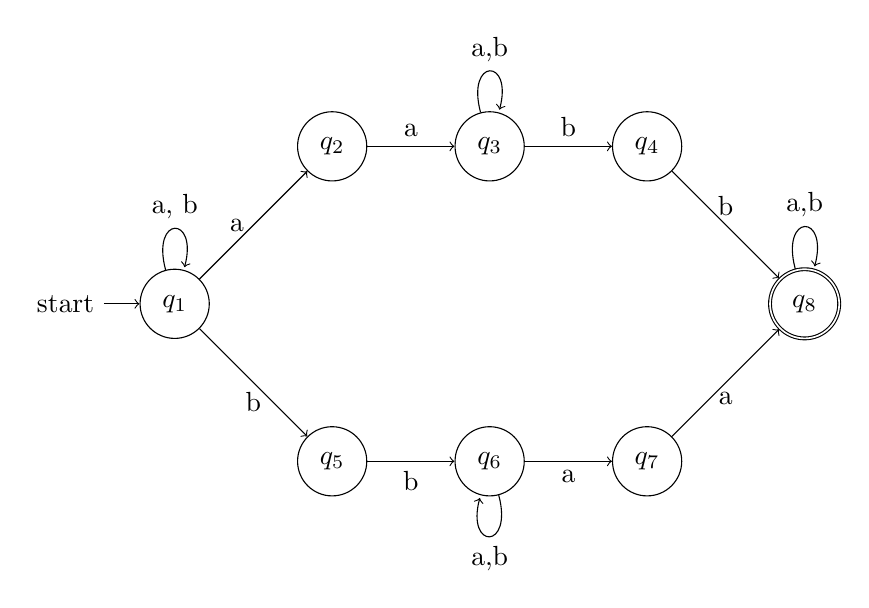
\begin{tikzpicture}
		\node[state, initial] (q1) at (0, 0) {$q_1$};
		\node[state] (q2) at (2, 2) {$q_2$};
		\node[state] (q3) at (4, 2) {$q_3$};
		\node[state] (q4) at (6, 2) {$q_4$};
		\node[state] (q5) at (2, -2) {$q_5$};
		\node[state] (q6) at (4, -2) {$q_6$};
		\node[state] (q7) at (6, -2) {$q_7$};
		\node[state, accepting](q8) at (8, 0) {$q_8$};

		\draw[->] (q1) edge[loop above] node{a, b} (q1);
		\draw[->] (q1) edge[above, left=0.2] node{a} (q2);
		\draw[->] (q1) edge[below] node{b} (q5)
				  (q2) edge[above] node{a} (q3)
				  (q5) edge[below] node{b} (q6)
				  (q6) edge[loop below] node{a,b} (q6)
				  (q6) edge[below] node{a} (q7)
				  (q7) edge[below] node{a} (q8)
				  (q3) edge[loop above] node{a,b} (q3)
				  (q3) edge[above] node{b} (q4)
				  (q4) edge[above] node{b} (q8)
				  (q8) edge[loop above] node{a,b} (q8);
	\end{tikzpicture}
\end{center}
	
\subsection*{c)}
Let $M=(K, \Sigma, \Delta, s, F)$ be the nondeterministic finite automaton in the previous question and $M'=(K', \Sigma, \delta, s', F')$ be the deterministic equivalent of $M$. Then,
\begin{equation*}
	K' = 2^K
\end{equation*}
\begin{equation*}
	s' = E(s)
\end{equation*}
\begin{equation*}
	F' = \{Q \subseteq K \mid Q \cap F \neq \emptyset\} 
\end{equation*}
\begin{equation*}
	\delta (Q,a) = \bigcup\{E(p) \mid p \in K \land (q, a, p) \in \Delta \}
\end{equation*}

\begin{equation*}
	s' = E(s) = \{q_1\}
\end{equation*}

For $\{q_1\}$:
\begin{equation*}
	(q_1, a, q_1), (q_1, a, q_2) \in \Delta, \ \delta (\{q_1\}, a) = E(q_1) \cup E(q_2) = \{q_1, q_2\}
\end{equation*}
\begin{equation*}
	(q_1, b, q_1), (q_1, b, q_5) \in \Delta, \ \delta (\{q_1\}, b) = E(q_1) \cup E(q_5) = \{q_1, q_5\}
\end{equation*}

For $\{q_1, q_2\}$:
\begin{equation*}
	(q_1, a, q_1), (q_1, a, q_2), (q_2, a, q_3) \in \Delta
\end{equation*}
\begin{equation*}
	\delta (\{q_1, q_2\}, a) = E(q_1) \cup E(q_2) \cup E(q_3) = \{q_1, q_2, q_3\}
\end{equation*}
\begin{equation*}
	(q_1, b, q_1), (q_1, b, q_5) \in \Delta, \ \delta (\{q_1, q_2\}, b) = E(q_1) \cup E(q_5) = \{q_1, q_5\}
\end{equation*}

For $\{q_1, q_5\}$:
\begin{equation*}
	(q_1, a, q_1), (q_1, a, q_2) \in \Delta, \ \delta (\{q_1, q_5\}, a) = E(q_1) \cup E(q_2) = \{q_1, q_2\}
\end{equation*}
\begin{equation*}
	(q_1, b, q_1), (q_1, b, q_5), (q_5, b, q_6) \in \Delta, \ \delta (\{q_1, q_5\}, b)
\end{equation*}

For $\{q_1, q_2, q_3\}$:
\begin{equation*}
	(q_1, a, q_1), (q_1, a, q_2), (q_2, a, q_3), (q_3, a, q_3) \in \Delta,
\end{equation*}
\begin{equation*}
	\delta (\{q_1, q_2, q_3\}, a) = E(q_1) \cup E(q_2) \cup E(q_3) = \{q_1, q_2, q_3\}
\end{equation*}
\begin{equation*}
	(q_1, b, q_1), (q_1, b, q_5), (q_3, b, q_3), (q_3, b, q_4) \in \Delta,
\end{equation*}
\begin{equation*}
	\delta (\{q_1, q_2, q_3\}, b) = E(q_1) \cup E(q_3) \cup E(q_4) \cup E(q_5) = \{q_1, q_3, q_4, q_5\}
\end{equation*}

For $\{q_1, q_5, q_6\}$:
\begin{equation*}
	(q_1, a, q_1), (q_1, a, q_2), (q_6, a, q_6), (q_6, a, q_7) \in \Delta,
\end{equation*}
\begin{equation*}
	\delta (\{q_1, q_5, q_6\}, a) = E(q_1) \cup E(q_2) \cup E(q_6) \cup E(q_7) = \{q_1, q_2, q_6, q_7\}
\end{equation*}
\begin{equation*}
	(q_1, b, q_1), (q_1, b, q_5), (q_5, b, q_6), (q_6, b, q_6) \in \Delta,
\end{equation*}
\begin{equation*}
	\delta (\{q_1, q_5, q_6\}, b) = E(q_1) \cup E(q_5) \cup E(q_6) = \{q_1, q_5, q_6\}
\end{equation*}

For $\{q_1, q_3, q_4, q_5\}$:
\begin{equation*}
	(q_1, a, q_1), (q_1, a, q_2), (q_3, a, q_3) \in \Delta 
\end{equation*}
\begin{equation*}
	\delta (\{q_1, q_3, q_4, q_5\}, a) = E(q_1) \cup E(q_2) \cup E(q_3) = \{q_1, q_2, q_3\}\\
\end{equation*}
\begin{equation*}
	(q_1, b, q_1), (q_1, b, q_5), (q_3, b, q_3), (q_3, b, q_4), (q_4,b,q_8), (q_5, b, q_6) \in \Delta, 
\end{equation*}
\begin{equation*}
	\delta (\{q_1, q_3, q_4, q_5\}, b) = E(q_1) \cup E(q_3), E(q_4) \cup E(q_5) \cup E(q_6) \cup E(q_8) = \{q_1, q_3, q_4, q_5, q_6, q_8\}
\end{equation*}

For $\{q_1, q_2, q_6, q_7\}$:
\begin{equation*}
	(q_1, a, q_1), (q_1, a, q_2), (q_2, a, q_3), (q_6, a, q_6), (q_6, a, q_7), (q_7, a, q_8) \in \Delta
\end{equation*}
\begin{equation*}
	\delta (\{q_1, q_2, q_6, q_7\}, a) =
\end{equation*}
\begin{equation*}
	 E(q_1) \cup E(q_2) \cup E(q_3) \cup E(q_6) \cup E(q_7) \cup E(q_8) = \{q_1, q_2, q_3, q_6, q_7, q_8\}
\end{equation*}

\begin{equation*}
	(q_1, b, q_1), (q_1, b, q_5), (q_6,b,q_6) \in \Delta
\end{equation*}
\begin{equation*}
	\delta (\{q_1, q_2, q_6, q_7\}, b) = E(q_1) \cup E(q_5) \cup E(q_6) = \{q_1, q_5, q_6\}
\end{equation*}

For $\{q_1, q_3, q_4, q_5, q_6, q_8\}$:
\begin{equation*}
	(q_1,a,q_1), (q_1, a, q_2), (q_3, a, q_3), (q_6, a, q_6), (q_6, a, q_7), (q_8, a, q_8) \in \Delta
\end{equation*}
\begin{equation*}
	\delta (\{q_1, q_3, q_4, q_5, q_6, q_8\}, a) = 
\end{equation*}
\begin{equation*}
	E(q_1) \cup E(q_2) \cup E(q_3) \cup E(q_6) \cup E(q_7) \cup E(q_8) = \{q_1, q_2, q_3, q_6, q_7, q_8\}
\end{equation*}
\begin{equation*}
	(q_1,b,q_1), (q_1, b, q_5), (q_3, b, q_3), (q_3, b, q_4), (q_4, b, q_8), (q_6, b, q_6), (q_8, a, q_8) \in \Delta
\end{equation*}
\begin{equation*}
	\delta (\{q_1, q_3, q_4, q_5, q_6, q_8\}, b) = 
\end{equation*}
\begin{equation*}
	E(q_1) \cup E(q_3), E(q_4) \cup E(q_5) \cup E(q_6) \cup E(q_8) = \{q_1, q_3, q_4, q_5, q_6, q_8\}
\end{equation*}

For $\{q_1, q_2, q_3, q_6, q_7, q_8\}$:
\begin{equation*}
(q_1, a, q_1), (q_1, a, q_2), (q_2, a, q_3), (q_3, a, q_3), (q_6, a, q_6), 
\end{equation*}
\begin{equation*}
	(q_6, a, q_7), (q_7, q, q_8), (q_8, a, q_8) \in \Delta
\end{equation*}
\begin{equation*}
	\delta (\{q_1, q_2, q_3, q_6, q_7, q_8\}, a) = 
\end{equation*}
\begin{equation*}
	E(q_1) \cup E(q_2) \cup E(q_3) \cup E(q_6) \cup E(q_7) \cup E(q_8) = \{q_1, q_2, q_3, q_6, q_7, q_8\}
\end{equation*}
\begin{equation*}
	(q_1, b, q_1), (q_1, b, q_5), (q_3, b, q_3), (q_3, b, q_4) (q_6, b, q_6), (q_8, b, q_8) \in \Delta
\end{equation*}
\begin{equation*}
	\delta (\{q_1, q_2, q_3, q_6, q_7, q_8\}, b) = 
\end{equation*}
\begin{equation*}
	E(q_1) \cup E(q_3), E(q_4) \cup E(q_5) \cup E(q_6) \cup E(q_8) = \{q_1, q_3, q_4, q_5, q_6, q_8\}
\end{equation*}

\begin{center}
	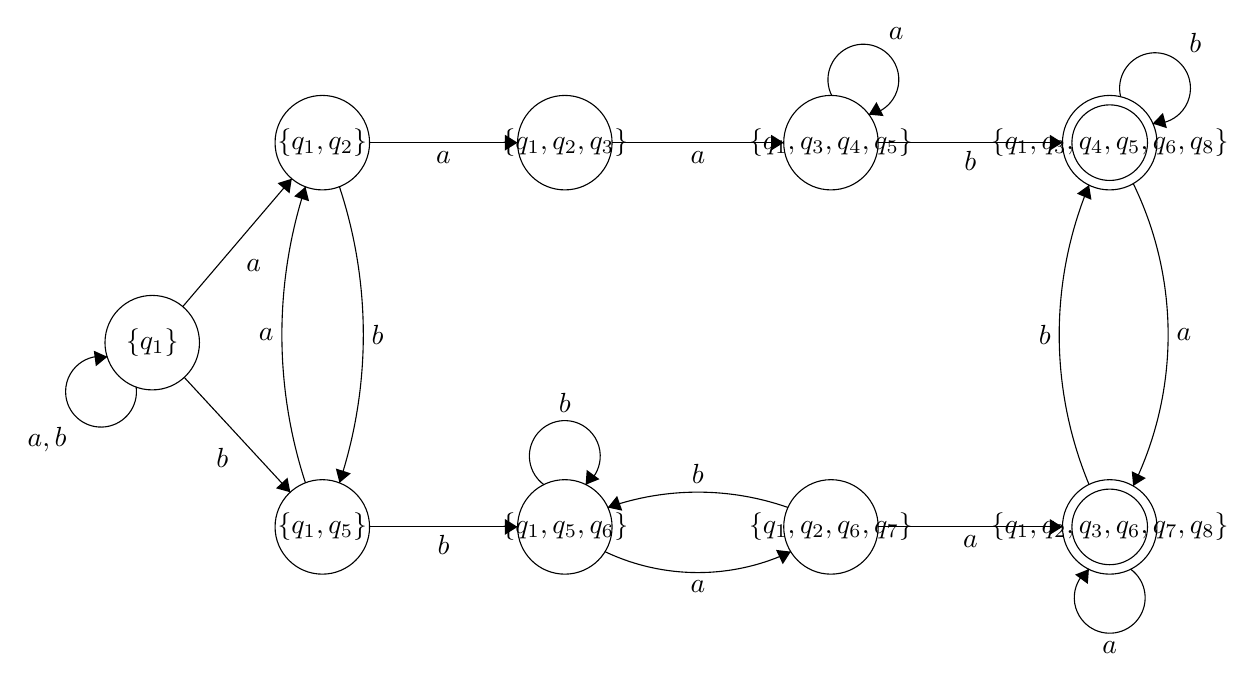
\begin{tikzpicture}[scale=0.2]
		\tikzstyle{every node}+=[inner sep=0pt]
		\draw [black] (9.7,-21.2) circle (3);
		\draw (9.7,-21.2) node {$\{q_1\}$};
		\draw [black] (20.5,-8.5) circle (3);
		\draw (20.5,-8.5) node {$\{q_1,q_2\}$};
		\draw [black] (35.9,-8.5) circle (3);
		\draw (35.9,-8.5) node {$\{q_1,q_2,q_3\}$};
		\draw [black] (52.8,-8.5) circle (3);
		\draw (52.8,-8.5) node {$\{q_1,q_3,q_4,q_5\}$};
		\draw [black] (70.5,-8.5) circle (3);
		\draw (70.5,-8.5) node {$\{q_1,q_3,q_4,q_5,q_6,q_8\}$};
		\draw [black] (70.5,-8.5) circle (2.4);
		\draw [black] (20.5,-32.9) circle (3);
		\draw (20.5,-32.9) node {$\{q_1,q_5\}$};
		\draw [black] (35.9,-32.9) circle (3);
		\draw (35.9,-32.9) node {$\{q_1,q_5,q_6\}$};
		\draw [black] (52.8,-32.9) circle (3);
		\draw (52.8,-32.9) node {$\{q_1,q_2,q_6,q_7\}$};
		\draw [black] (70.5,-32.9) circle (3);
		\draw (70.5,-32.9) node {$\{q_1,q_2,q_3,q_6,q_7,q_8\}$};
		\draw [black] (70.5,-32.9) circle (2.4);
		\draw [black] (11.64,-18.91) -- (18.56,-10.79);
		\fill [black] (18.56,-10.79) -- (17.66,-11.07) -- (18.42,-11.72);
		\draw (15.65,-16.29) node [right] {$a$};
		\draw [black] (11.73,-23.4) -- (18.47,-30.7);
		\fill [black] (18.47,-30.7) -- (18.29,-29.77) -- (17.56,-30.45);
		\draw (14.57,-28.51) node [left] {$b$};
		\draw [black] (19.429,-30.099) arc (-161.90863:-198.09137:30.268);
		\fill [black] (19.43,-11.3) -- (18.71,-11.91) -- (19.66,-12.22);
		\draw (17.43,-20.7) node [left] {$a$};
		\draw [black] (8.678,-24.008) arc (7.73869:-280.26131:2.25);
		\draw (4.29,-27.34) node [left] {$a,b$};
		\fill [black] (6.85,-22.1) -- (5.99,-21.71) -- (6.12,-22.7);
		\draw [black] (21.586,-11.295) arc (18.34603:-18.34603:29.879);
		\fill [black] (21.59,-30.1) -- (22.31,-29.5) -- (21.36,-29.19);
		\draw (23.6,-20.7) node [right] {$b$};
		\draw [black] (23.5,-8.5) -- (32.9,-8.5);
		\fill [black] (32.9,-8.5) -- (32.1,-8) -- (32.1,-9);
		\draw (28.2,-9) node [below] {$a$};
		\draw [black] (23.5,-32.9) -- (32.9,-32.9);
		\fill [black] (32.9,-32.9) -- (32.1,-32.4) -- (32.1,-33.4);
		\draw (28.2,-33.4) node [below] {$b$};
		\draw [black] (34.577,-30.22) arc (234:-54:2.25);
		\draw (35.9,-25.65) node [above] {$b$};
		\fill [black] (37.22,-30.22) -- (38.1,-29.87) -- (37.29,-29.28);
		\draw [black] (50.251,-34.471) arc (-64.60001:-115.39999:13.758);
		\fill [black] (50.25,-34.47) -- (49.31,-34.36) -- (49.74,-35.27);
		\draw (44.35,-36.3) node [below] {$a$};
		\draw [black] (55.8,-32.9) -- (67.5,-32.9);
		\fill [black] (67.5,-32.9) -- (66.7,-32.4) -- (66.7,-33.4);
		\draw (61.65,-33.4) node [below] {$a$};
		\draw [black] (38.9,-8.5) -- (49.8,-8.5);
		\fill [black] (49.8,-8.5) -- (49,-8) -- (49,-9);
		\draw (44.35,-9) node [below] {$a$};
		\draw [black] (52.85,-5.512) arc (206.76814:-81.23186:2.25);
		\draw (56.94,-1.99) node [above] {$a$};
		\fill [black] (55.2,-6.72) -- (56.14,-6.81) -- (55.69,-5.92);
		\draw [black] (55.8,-8.5) -- (67.5,-8.5);
		\fill [black] (67.5,-8.5) -- (66.7,-8) -- (66.7,-9);
		\draw (61.65,-9) node [below] {$b$};
		\draw [black] (38.63,-31.666) arc (109.3436:70.6564:17.268);
		\fill [black] (38.63,-31.67) -- (39.55,-31.87) -- (39.22,-30.93);
		\draw (44.35,-30.19) node [above] {$b$};
		\draw [black] (71.198,-5.594) arc (194.2172:-93.7828:2.25);
		\draw (75.94,-2.82) node [above] {$b$};
		\fill [black] (73.23,-7.29) -- (74.13,-7.58) -- (73.88,-6.61);
		\draw [black] (71.995,-11.098) arc (25.99023:-25.99023:21.911);
		\fill [black] (71.99,-30.3) -- (72.79,-29.8) -- (71.9,-29.36);
		\draw (74.71,-20.7) node [right] {$a$};
		\draw [black] (69.186,-30.205) arc (-157.47051:-202.52949:24.807);
		\fill [black] (69.19,-11.19) -- (68.42,-11.74) -- (69.34,-12.13);
		\draw (66.79,-20.7) node [left] {$b$};
		\draw [black] (71.823,-35.58) arc (54:-234:2.25);
		\draw (70.5,-40.15) node [below] {$a$};
		\fill [black] (69.18,-35.58) -- (68.3,-35.93) -- (69.11,-36.52);
	\end{tikzpicture}
\end{center}

\subsection*{d)}
For NFA:
\begin{equation*}
	(q_1, bbabb) \vdash_M (q_5, babb) \vdash_M (q_6, abb) \vdash_M (q_6, bb) \vdash_M (q_6, b) \vdash_M (q_6,e)
\end{equation*}
\newline
For DFA:
\begin{equation*}
	(\{q_1\}, bbabb) \vdash_{M'} (\{q_1, q_5\}, babb) \vdash_{M'} (\{q_1, q_5, q_6\} abb) \vdash_{M'} 
\end{equation*}
\begin{equation*}
	(\{q_1, q_2, q_6, q_7\}, bb) \vdash_{M'} (\{q_1, q_5, q_6\}, b) \vdash_{M'} (\{q_1, q_5, q_6\},e)
\end{equation*}
Since string $"bbabb"$ does not lead to any final state, it is not accepted by the automatons.
\section*{Q2}
\subsection*{a)}
Assume $L_1$ is a regular languge. Then by the pumping lemma for any string $w \in L_1$ with $\mid w \mid \geq n$ can be written as $w = xyz$ such that $y \neq e$, $\mid xy \mid \leq n$ and $xy^iz \in L_1$ for each $i \geq 0$.
Let's choose string $w = a^kb^l$ where $k > l$. Let $w = xyz$ since $|w| \geq k $ then $|xy|$ must be less or equal to $k$. $y$ can be represented as $a^s$ where $s \leq k$. Then for $i=0$, string $x(a^s)^iz = xz = a^{k-s}b^l \notin L_1$ contradicts the theorem, therefore $L_1$ is not regular.
Since $L_1$ is not regular, because of the closure properties of regular languages $L_2$ is not also a regular language.
\subsection*{b)}
$L_5$ includes all strings starting with any number of $a$'s followed by any number of $b$'s. On the other hand $L_4$ only includes strings starting with any number of $a$'s followed by same number of $b$'s. Therefore $L_4$ is a subset of $L_5$. Then, $L_4 \cup L_5 = L_5$. $L_5$ can also be written as $L_5 = a^*b^*$. Since $L_5$ can be written in form of regular expressions it is a regular language. $L_6$ is written in form of regular expressions, therefore $L_6$ is also a regular language.
\begin{equation*}
	L_4 \cup L_5 \cup L_6 = L_5 \cup L_6
\end{equation*}
By the closure properties of regular languages, if $L_5$ and $L_6$ is regular then $L_5 \cup L_6$ must be regular. 
\end{document}